\section{Beam diagnostic at ESS}

\begin{frame}
  \frametitle{Beam diagnostic}
  Eye of the accelerator
  Beam diagnostics are mandatory tools
  \begin{itemize}
    \item Beam position, beam current, beam energy, beam losses ...
    \item
  \end{itemize}

  \begin{block}{Beam diagnostics at ESS}
    \begin{itemize}
      \item 15 different systems
      \item A total of 480 beam diagnostic devices will be installed along the accelerator.
    \end{itemize}
  \end{block}

  Today, we are presenting a device that measure the transverse beam profile:

  \begin{block}{Definition}
    Spacial distribution of the charges of the beam in the transverse plane.
    \begin{itemize}
      \item Beam shape
      \item Beam position
      \item Relative beam amplitude
    \end{itemize}
  \end{block}

  In fact at ESS, the transverse profile measurement is done by 3 different types of devices. We are in charge of just one of them.

\end{frame}

\begin{frame}
  \frametitle{Profile measurement method}
  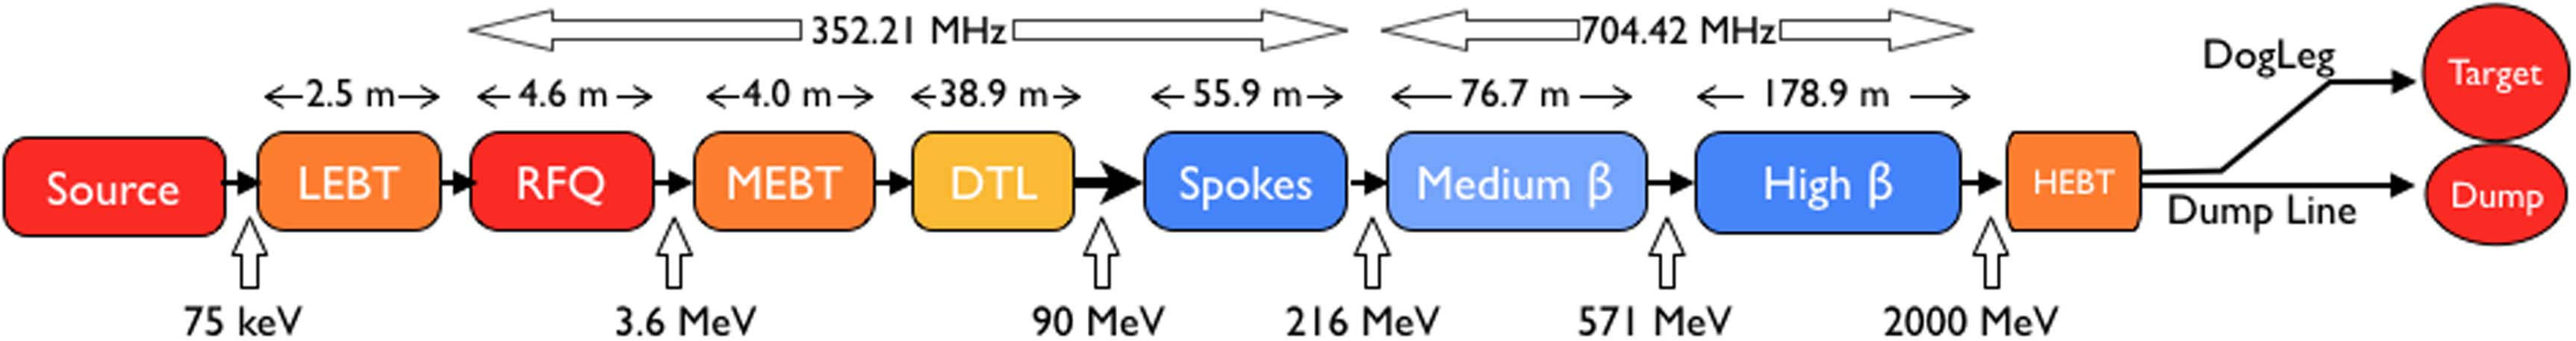
\includegraphics[width=\textwidth]{01_Neutron/fig/fig000_ESS_acc}
  \begin{columns}
    \begin{column}{0.45\textwidth}
      \begin{block}{Wire Scanner/SEM Grid}
        Measurement of the secondaries electrons or hadronic cascade emitted during the collision of proton with one or more wires.
      \end{block}
      \begin{block}{Pro/cons}
        \begin{itemize}
          \item[+] High sensitivity
          \item[-] Interceptive measurement
        \end{itemize}
      \end{block}
    \end{column}
    \begin{column}{0.45\textwidth}
      Image/Schema
      \begin{block}{Use at ESS}
        \begin{itemize}
          \item Everywhere along accelerator
          \item But limited to low duty cycle
        \end{itemize}
      \end{block}
    \end{column}
  \end{columns}
  \begin{alertblock}{Wire scanners cannot work at nominal conditions}
    The WS can not withstand the $5\,\mathrm{MW}$ beam power. Wire can melt and may compromise the SC cavities.
  \end{alertblock}
\end{frame}

\begin{frame}
  \frametitle{Profile measurement method}
  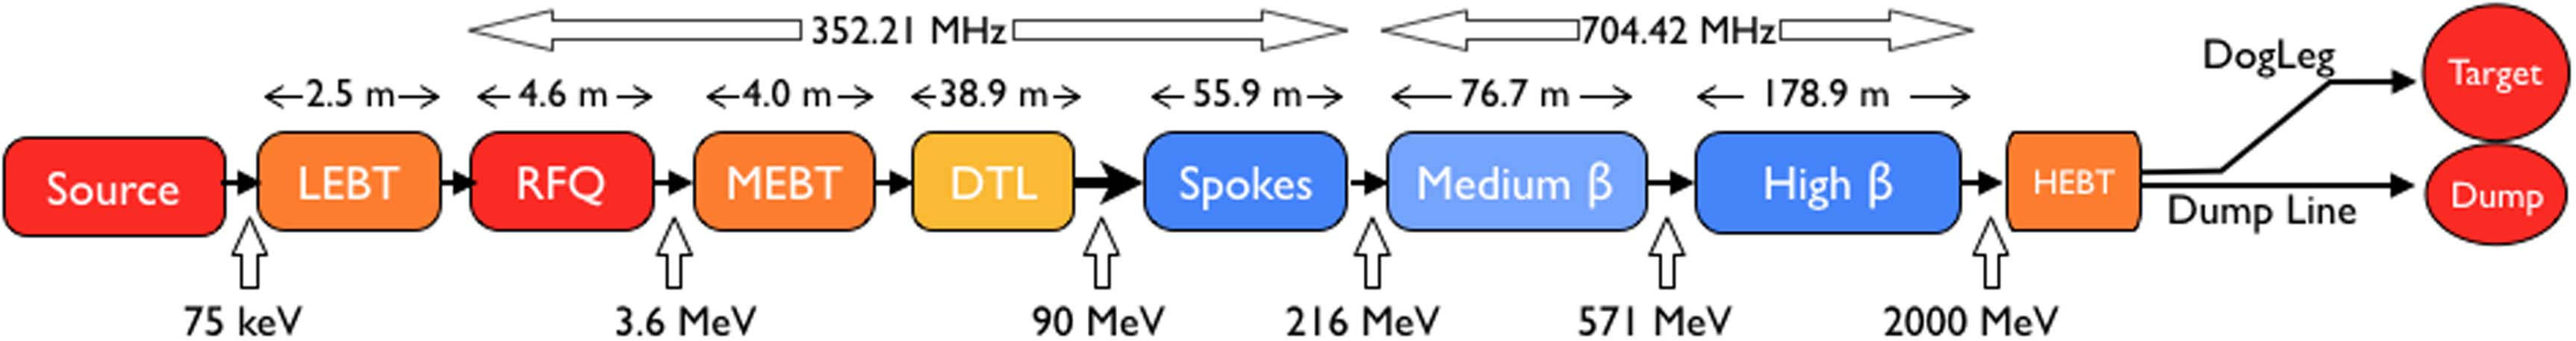
\includegraphics[width=\textwidth]{01_Neutron/fig/fig000_ESS_acc}
  \begin{columns}
    \begin{column}{0.45\textwidth}
      \begin{block}{FPM}
        Measurement of the fluorescence induced by the beam.
      \end{block}
      \begin{block}{Pro/cons}
        \begin{itemize}
          \item[+] Non-invasive
          \item[+] No active elements in vacuum
          \item[-] $4\pi$ solid angle
          \item[-] Depends on vacuum
        \end{itemize}
      \end{block}
    \end{column}
    \begin{column}{0.45\textwidth}
      Image/Schema
      \begin{block}{Use at ESS}
        \begin{itemize}
          \item In the hot parts of the accelerator
          \item At low duty cycle
        \end{itemize}
      \end{block}
    \end{column}
  \end{columns}
  \begin{alertblock}{FPM cannot work in superconducing part}
    In the cryogenic section, the pressure is too low for FPM (expected $10^{-9}\,\mathrm{mbar}$)
  \end{alertblock}
\end{frame}

\begin{frame}
  \frametitle{IPM}
  \begin{alertblock}{So no profile measurement in SC part at nominal condition?}

  \end{alertblock}
  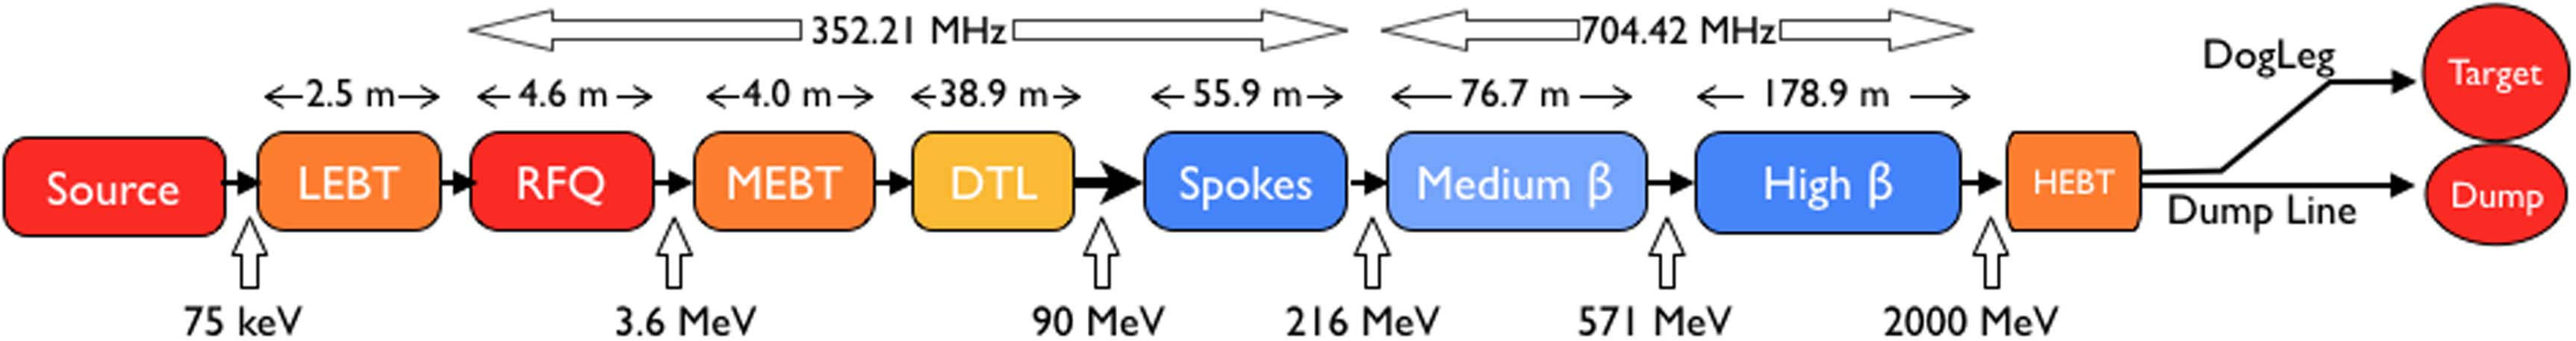
\includegraphics[width=\textwidth]{01_Neutron/fig/fig000_ESS_acc}

  \begin{columns}
    \begin{column}{0.45\textwidth}
      \begin{block}{How it works}
        \begin{enumerate}
          \item Beam protons pass through the residual gas, inducing ionizations: $e^-$/ion pairs.
          \item An electric field drives $e^-$ or ions towards a segmented readout system.
          \item Profile in one transverse direction. Complete profile: pair of IPMs.
        \end{enumerate}
      \end{block}
    \end{column}
    \begin{column}{0.45\textwidth}
      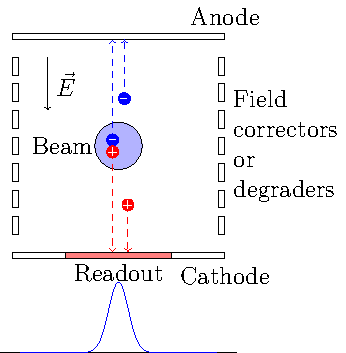
\includegraphics[width=\textwidth]{02_ESS/fig/fig000_IPM.pdf}
    \end{column}
  \end{columns}
\end{frame}

\begin{frame}
  \frametitle{IPM}
  \begin{columns}[T]
    \begin{column}{0.45\textwidth}
      \begin{block}{Fission reactor}
        \begin{itemize}
          \item Uses fission reaction.
        \end{itemize}    
      \end{block}
      \vfill
    \end{column}
    \begin{column}{0.45\textwidth}
      \begin{block}{Spallation source}
        \begin{itemize}
          \item Uses particle accelerator
        \end{itemize}        
      \end{block}
      \vfill
    \end{column}
  \end{columns}
  \begin{block}{History}
    \begin{itemize}
      \item 1960-1970:
      \item 1990-2000:
      \item 201
      \item As well, constant improvement of and simulations
    \end{itemize}
  \end{block}
  IPM are popular on proton circular accelerator or storage ring:
  \begin{itemize}
    \item Where can be extremely low (below $10^{-10}\,\mathrm{}$)
    \item 
  \end{itemize}
  \begin{alertblock}{The use of }
    Can we use IPMs in the superconducting part of the ESS accelerator?
  \end{alertblock}
\end{frame}